\section{Introduction}
\label{sec:intro}

\mwh{I think we need to cut a page from the intro. This is too long
  and it's too hard to tell what we are contributing.}

%%%%%%%%%%%%%%%%%%%%%%%%%%%%%%%%%%%%%%%%%%%%%%%%%%%%%%%%%%%%
%%% 1. The first paragraph should discuss why we should care about quantum computers/quantum programming languages. Use Grover's search/Shor's algorithms as examples of showing quantum supremacy.

Quantum computers offer unique capabilities that can be used to
program substantially faster algorithms compared to those written for
classical computers. For example, Grover's search algorithm \cite{grover1996,grover1997}
can query unstructured data in sub-linear time (compared to linear
time on a classical computer), and Shor's algorithm \cite{shors} can factorize a
number in polynomial time (compared to sub-exponential time for the
best known classical algorithm). 

%%%%%%%%%%%%%%%%%%%%%%%%%%%%%%%%%%%%%%%%%%%%%%%%%%%%%%%%%%%%
%%% 2a. Challenge: hard to test and debug quantum programs and tools
% (e.g., compilers).

A major challenge today is \emph{reasoning that quantum programs implement
the intended algorithm correctly and efficiently.}
Quantum programs are typically expressed as \emph{circuits} comprising
a variety of \emph{quantum gates} each applied to one or more
\emph{quantum bits} (qubits). 
\mwh{Dropped mention of quipper etc. and metaprograms -- move to background?}
% Circuits 
% are often built by meta-programs embedded in a host language, e.g.,
% Python (for Qiskit~\cite{Qiskit}, Cirq~\cite{cirq}, PyQuil~\cite{PyQuil}, and others) or Haskell (for
% Quipper~\cite{Green2013}). 
Testing quantum programs on actual quantum computers is difficult.
Few computers exist, and those that do have limited resources---at most 10s of qubits \cite{quantumcomputercurrent1,quantumcomputercurrent2}, 
and those qubits are unreliable, tending to decohere after just a few gate applications. 
Furthermore, quantum algorithms are often probabilistic, which
means that an incorrect answer could owe to
randomness, noise, or algorithmic mistakes. Debugging is also hard:
measuring (observing) a quantum state may change it. 
Some of these problems can be addressed by simulating quantum
programs on classical computers, but doing so
is generally intractable. The size of a quantum state is, at worst,
exponential in the number of qubits, meaning that a program that uses
50 or more qubits may be impossible to simulate on even the most powerful
of classical machines.

% I think the point of the (commented) paragraph below is that choosing between different implementations of quantum circuits is hard -- but I don't think this is directly addressed by VQO. -Kesha

% Selecting the most efficient circuit for a specific usage is an even harder task.
% Many quantum algorithms, acting as sub-components of large algorithms, only have brief "semantics" on paper and the semantics might be slightly different with different implementations, because quantum algorithms are mostly probabilistic. 
% For example, there are at least three different
% kinds of \emph{Approximate quantum Fourier transform} (AQFT) implementations \cite{ApproximateQFT,appox-qft2,appox-qft1}, and each of them has slightly different semantics.
% Testing their exact meaning is hard based on the current quantum computer situation,
% and analyzing their suitability and creating an efficient quantum circuit with the "right" implementation choice of these sub-components are even harder but essential in near term quantum circuits.
% For example, we have found AQFT is not suitable in addition circuits (\Cref{sec:qft-case}), but it is efficient to implement a modulo operation circuit with AQFT sub-components.

%%%%%%%%%%%%%%%%%%%%%%%%%%%%%%%%%%%%%%%%%%%%%%%%%%%%%%%%%%%%
%%% 2b. Successful  approach: formal verification, and prior work on VOQC and SQIR (for proving correct source algorithms).

Recent work (surveyed by \citet{chareton2021formal}) proposes to address these problems using \emph{formal methods} to prove that an algorithm always does what it is intended to do.
\sqir, the \emph{Small Quantum Intermediate Representation}~\cite{PQPC}, is a circuit language embedded in the Coq proof
assistant that has been used to prove several standard quantum
algorithms correct, including Grover's and components of Shor's.
% SQIR programs are subject to optimization by
% VOQC, the \emph{Verified Optimizer for Quantum Circuits}, whose
% performance is on par with today's best unverified circuit
% optimizers~\cite{VOQC}.
\qbricks~\cite{qbricks}, \qwire~\cite{Rand2017}, and QHL~\cite{qhoare}
have also been used to prove quantum programs correct.
% and PyZX, QMDD, and Certiq have been
% used to prove optimizations correct. \mwh{CITES}

%%%%%%%%%%%%%%%%%%%%%%%%%%%%%%%%%%%%%%%%%%%%%%%%%%%%%%%%%%%%
% 3. (Like your para 2) But: SQIR, like all quantum circuit languages, is low-level. Key part of larger quantum programs is the oracle (say what an oracle is). E.g., 90% of Shor's is the oracle for mod-mult. Coding up large oracles by hand is both error prone (two bugs in QFT adder) and potentially inefficient.

A limitation of these prior works is that they have not verified
\emph{complete} quantum algorithms. They have ignored algorithms'
classical function parameters, which are called \emph{oracles}. For
example, Grover's algorithm is parameterized by a predicate function that determines
when the searched-for data is found. Shor's algorithm finds the period
of a classical modular exponentiation function, where the modulus is
the number being factored.  An important source of speedups in these
algorithms is the quantum computer's ability to apply the oracle
function \emph{coherently}, i.e., to a \emph{superposition} of
classical queries, thus carrying out in one step a function that would
potentially take many steps on a classical computer.
%
Oracles contribute a significant fraction of the final compiled circuit; e.g., Shor's
modular exponentiation component constitutes 90\% of the final
code~\cite{Gidney2021howtofactorbit}. 
\mwh{Potentially drop the following, or else find a better place to
  put it}
There are two tasks for reasoning about oracles. First,
to gain hoped-for assurances from the use of formal methods, we need
to verify \emph{all} of a quantum algorithm, including the (large) oracles it uses.
Second, for a near term quantum oracle, there are many implementations.
For example, there are many different quantum addition circuit implementations \cite{qft-adder,ripple-carry}. 
we need a fast development framework to permit the testing and evaluating,
in terms of circuit efficiency, of different implementations
and be able to select the best implementation in different circumstances. 

%%%%%%%%%%%%%%%%%%%%%%%%%%%%%%%%%%%%%%%%%%%%%%%%%%%%%%%%%%%%
% 4. What is OQASM and where does it fit in the solution for
% verifying/validating oracles

 To address this open problem, this paper presents \oqasm (pronounced
``O-chasm''), the \emph{oracle quantum assembly language}, 
whose aim is to make it easier to specify and either verify or test
efficient quantum oracles.
%
%%%%%%%%%%%%%%%%%%%%%%%%%%%%%%%%%%%%%%%%%%%%%%%%%%%%%%%%%%%%
% 5 Smaller, higher-level gateset than SQIR, sufficient for writing
% oracles but with more tractable means of assurance: Lack of
% entanglement means it's easier to do proofs, and feasible to perform
% testing/simulation. Prior work does not support quantum gates.
%
Because oracles are
classical functions, a reasonable approach would have been to design
\oqasm to be a circuit language comprised of classical gates; e.g.,
prior work has targeted gates \texttt{X} (``not''), \texttt{CNOT}
(``controlled not''), and \texttt{CCNOT} (``controlled controlled
not'', aka \emph{Toffoli}). Doing so would simplify proofs of
correctness and support efficient testing by simulation
because an oracle's behavior could be completely characterized by
its behavior on computational basis states (essentially, classical bitstrings). 
ReverC~\cite{reverC} and ReQWIRE~\cite{Rand2018ReQWIRERA} take
this approach. However, doing so cannot support optimized oracle
implementations that use fundamentally quantum functionality, e.g., as
in \emph{quantum Fourier transform} (QFT)-based arithmetic
circuits~\cite{qft-adder,2000quant}.
These circuits employ
quantum-native operations (e.g., controlled-phase operations) in the
\emph{QFT basis}, which is connected to the computational basis by QFT\@.
Our key insight is that expressing such optimizations does not require expressing
all quantum programs, as is possible in a language like \sqir. Instead,
\oqasm's type system restricts programs to those that admit
important optimizations while keeping simulation tractable. 

%%%%%%%%%%%%%%%%%%%%%%%%%%%%%%%%%%%%%%%%%%%%%%%%%%%%%%%%%%%%
% 6: Explain PQASM's basic setup here. Phase space, virtual qubits

% - Phase spaces. State is map from qubits to superposed values, tagged
% with the phase space they are part of.
% - Computational space and QFT space, sub-Hilbert etc.
% - Virtual qubits

\oqasm has two key features.
% First, its type system enforces that quantum states always consist of
% qubits that are in forms similar to the computational basis or the
% dual basis.  The type of gates that could be applied to the type of
% qubits are restricted by specially designed typing rule so that
% unentangled qubits never becomes \emph{entangled} after executing
% \oqasm programs. 
First, its type system
enforces that quantum states always consist of qubits that are easily
represented in either the computational basis or the QFT basis, and that they remain \emph{unentangled}. 
% The type of gates that could be applied to the type of qubits are restricted by
% specially designed typing rule so that unentangled qubits never
% becomes \emph{entangled} after executing \oqasm programs.
%Which gates may be applied to
%which qubits, and the effect of doing so, depends on the qubits'
%current phase space. The net benefit is that \oqasm
%qubits never become \emph{entangled}
Entanglement is the source of
exponential blowup that makes proof difficult and simulation
intractable.
In particular, representing an $n$-qubit \oqasm quantum state
takes $O(n)$ space, rather than $O(2^n)$, as in the general case.
Nevertheless, \oqasm quantum states can still be in
\emph{superposition}, which makes them more expressive than
classical states.

Second, \oqasm provides support for \emph{virtual qubit
management}. An \oqasm variable $x$ may refer to a \emph{group} of qubits,
e.g., that implement a binary-encoded number, while individual qubits
can be extracted via a relative offset, e.g., $(x,0)$ refers to $x$'s
first qubit. \oqasm provides position-shifting operations on
variables to left- or right-shift their underlying qubits, or
reverse their order---all useful for implementing arithmetic
operations. \oqasm's type system ensures that position shifting
requires no \texttt{SWAP} gates when compiled to \sqir, so there is no
added run-time cost. 

% 7. Results:
% Built a compiler from PQASM to SQIR and verified it correct
% (para 6 in part) Developed proved-correct implementations of arithmetic operators, operator --> PQASM (right?). These operators are efficient -- compare to alternatives
% (para 6 in part) Built a simulator for PQASM programs, with which we randomly test operators, which provides some assurance that operator implementations are correct (found bugs!)
% (your para 8, a little) Built a higher-level language called QIMP from which we compile to PQASM. QIMP uses partial evaluation to optimize the compilation process. More efficient than operator compilation in Quipper in some cases (say when)
% (para 9) Developed a version of Grover's algorithm that is completely
% proved correct. Framework in SQIR, with the oracle developed in
% PQASM. Other stuff?

\begin{figure}[t]
  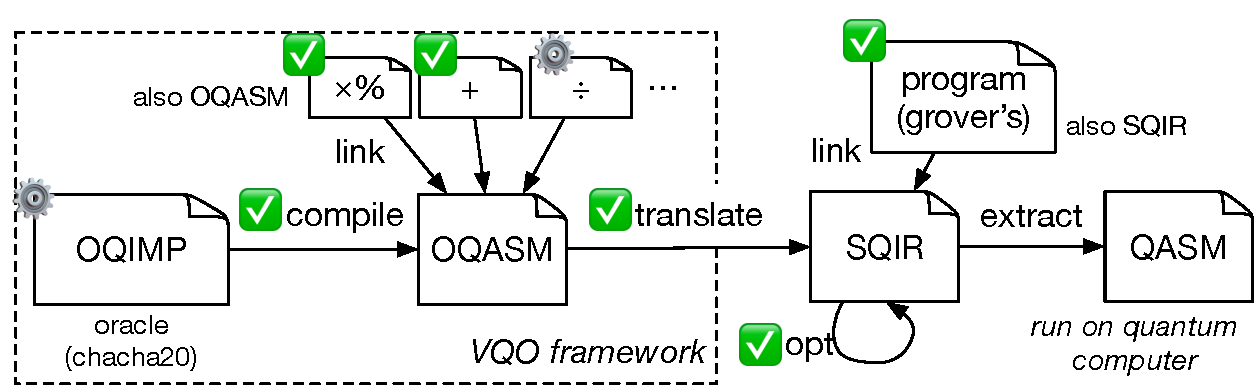
\includegraphics[width=2.8in]{qvm-arch}
  \caption{The \qvm high-assurance compiler stack. (Checkbox means
    formally verified; gear means property-tested.)}
\label{fig:arch}
\end{figure}

We have implemented \oqasm as part of a high-assurance compiler stack
called \qvm, for \emph{Quantum Verified Machine}, shown in \Cref{fig:arch}. 
The focus of this paper has been to build \name, the
\emph{Verified Quantum Oracle} framework, shown at the top.
An oracle can be specified in a simple, high-level programming language we call
\vqimp, which has standard imperative features and allows describing arbitrary 
classical programs, but distinguishes quantum
variables from classical parameters, allowing the latter to be
\emph{partially evaluated}~\cite{partialeval} during compilation to \oqasm.
\khh{We need to say that we're not limited to implementing arithmetic oracles (we also support sine and cosine). Is my minor addition to the previous sentence sufficient?}
\liyi{add including to show that arithemtic operations can mean a lot of things. }
The generated code links against implementations of standard arithmetic
operators including addition, multiplication, division, modulo, different comparison, sine, cosine, and exponentiation operations etc, also written in \oqasm. The \oqasm oracle is then translated
to \sqir, at which point it can be linked with a quantum program that
uses it. The complete \sqir program can be optimized using
\voqc~\cite{VOQC}, a proved-correct quantum circuit optimizer, and extracted
to OpenQASM 2.0 \cite{Cross2017} to run on a real quantum machine, if
desired.
We implemented \name in the Coq proof assistant, and \emph{certified}
(i.e., formally verified) that both compilation from \vqimp to \oqasm
and translation from \oqasm to \sqir are correct, i.e., the target
program's semantics provably match those of the source. 

To permit designing efficient quantum oracles, we implemented a \emph{property-based random testing} (PBT) framework for
\oqasm programs using QuickChick~\cite{quickchick}.
\mwh{Again, the following is long and not so clear to me.}
Based on the PBT framework, we provide a general development strategy for users to design efficient quantum oracle circuits, named \texttt{probability test-driven development}.
It allows users to effectively test oracle circuits
and probabilistically test an approximate oracle circuit with approximate sub-components with respect to the standard implementation of the circuit. 
With the fast testing results, we can then compare the circuit efficiency by compiling different circuits to \sqir/openQASM to find out the qubit and gate counts.
Prior to (or rather than) proving that an operator implementation matches its
specification, PBT can be used to attempt to automatically find
counterexamples to the correctness claim. PBT can also be used to test
oracles implemented in \vqimp by compiling them to \oqasm and testing
them against an \oqasm specification.

We have used \name to build several efficient oracles and oracle
components, and have either tested or proved their correctness.
\khh{TODO: Update this list based on experiment results}
\begin{itemize}
\item We have implemented a variety of arithmetic operators in \oqasm,
including QFT-, approximate QFT- and Toffoli-based multiplication, addition, modular
multiplication, and modular division. Overall,
circuit sizes are competitive with, and oftentimes better than, those
produced by Quipper~\cite{Green2013}, a state-of-the-art 
quantum programming framework.  Qubit
counts for the final QFT-based circuits often lower, sometimes
significantly so, compared to the Toffoli-based circuits. 
\khh{Likely cut the following:} We find
that \oqasm's virtual qubits reduce gate counts by 20\% compared to
using physical qubits and \texttt{SWAP} gates, even after \voqc optimization,
for our modular multiplier. 

\item We have proved correct both QFT and Toffoli-based adders, and QFT
and Toffoli-based modular multipliers (which are used in Shor's
algorithm). These constitute the first proved-correct implementations
of these functions, as far as we are aware.
To the best of out knowledge, this is the first time one provides a correctness certifications in a proof engine for any QFT-based arithmetic circuits.

\item We used PBT to test the correctness of various \oqasm operators.
Running 10,000 generated tests on 8- or 16-bit versions
of the operators takes just a few seconds. Testing 60-bit versions of
adders and multipliers takes just a few minutes, whereas running a general
quantum simulator on the final circuits fails \khh{True?} \liyi{yes. Yuxiang had tested it last time}.
To the best of our knowledge, this is the first time one can randomly test large quantum circuits in a reasonable time frame.
 We found several interesting bugs in the process
of doing PBT and proof, including in the original algorithmic
description of the QFT-based modular multiplier~\cite{qft-adder}.  

\item We use a general procedure (the probability test-driven development precedure) based on PBT to analyze the difference between QFT and approximate QFT (AQFT) circuits, and the suitability of AQFT in different algorithms.
We find out the AQFT-based approximate addition circuit does not provide good addition results, but the outputs have some portions that match the result of the same portions in a QFT-based addition circuit. 
We then utilize the AQFT-based approximate addition circuit to construct a
quantum modulo circuit, showing that this provides \khh{... TODO}
To the best of our knowledge, this is the best quantum modulo circuit implementation.

\item With \vqimp we have implemented sine, cosine, and other geometric functions
used in Hamiltonian
simulation~\cite{feynman1982simulating}, leveraging the arithmetic
circuits described above.
Compared to a sine function implemented in Quipper, \name's uses far 
fewer qubits thanks to \vqimp's partial evaluation.

\item Finally, to put all of the pieces together, we implemented the
  ChaCha20 stream cipher \cite{chacha} in \vqimp and used it as an oracle for
  Grover's search, previously implemented and proved correct in \sqir~\cite{PQPC}. We used PBT to test
  the oracle's correctness. Combining its tested
  property with Grover's correctness property, we demonstrate that Grover's is able to
  invert the ChaCha20 function and find collisions.
\end{itemize}

We begin with some background on quantum computing (\Cref{sec:background}) and then
present \oqasm's syntax, typing, and semantics (\Cref{sec:vqir}). Then we
discuss \name's implementation: \oqasm's translator and property-based
tester, and \vqimp (\Cref{sec:implementation}). Finally, we present our results
(\Cref{sec:evaluation,sec:case-study}), compare against related work (\Cref{sec:related}), and conclude. All
code presented in this paper is freely available (URL redacted).


\ignore{
\liyi{Added:}

One important feature of quantum programs is entanglement, which users utilize the movement of small particles to control the behaviors of the whole quantum array. An analogy of the entanglement feature is to drop an ink drop in a large pool of water so that the black is transmitted to the whole pool. Learning about if two qubit arrays are entangled can be beneficial to quantum program analysis. For example, quantum separation logic \cite{quantumseparation} requires the state can be separated into two parts only if they are not entangled. In terms of physical quantum computer implementation, entanglement is not only a feature but also an important resources that must be used efficiently. For example, in the development of quantum Fourier transform (QFT) \cite{ApproximateQFT}, researchers tried many different circuit models, and reached a best circuit model \cite{coppersmith2002approximate}, which is widely used today. The key feature of the model decoheres entanglement among different qubits (meaning that if the input is not superposition qubits, then the circuit does not create entanglement), which in fact makes physical circuit implementation a lot easier.
Unfortunately, entanglement detection is at least an NP-hard problem \cite{entanglementdetection}, and most likely in the exponential class, it is impractical to analyze the local property of a quantum program by detecting if two qubits arrays are entangled.

In \name, we carefully investigate no the situation of when a quantum gate does not cause entanglement and form circuit languages with a type system to enforce the non-entanglement property in evaluating quantum programs. It allows us to easily analyze quantum programs, especially oracle circuits. The analysis is not only about the circuit correctness but also about a possibility of selecting the best circuit implementation with the least usage of quantum gates and qubits, through automatic circuit reasoning by randomized testing.
In doing so, we develop two kinds of circuit IR language. The first one, \oqasm, is a language to describe quantum oracles. In near term quantum circuits, oracles typically describe arithmetic circuits, such as arithmetic operations and arithmetic comparison circuits.
\oqasm is capable of defining all of the popular arithmetic circuits. Through the randomized testing framework, for a particular arithmetic operation, we are able to evaluate the correctness and efficiency of different circuits, and select the best one.
The second one, \pqasm, is built on top of \oqasm by dropping the reversibility. The observation is that, if we split many quantum algorithms, such as Quantum Phase Estimation (QPE) \cite{kitaev1995quantum}, into small pattern components, the qubit arrays are not entangled provided that the inputs are all classical values (different bitstring combinations of $\ket{0}$ and $\ket{1}$). 
In the QFT (approximate QFT) circuit in \Cref{fig:background-circuit-example}, if the input is bitstring of $\ket{0}$ and $\ket{1}$, the output is a superposition state without entanglement. The analysis is valuable because we can split out sub-quantum components now and analyze it by using classical computer tools such as randomized testing, and we have simple pre-proved predicate to connect the sub-components with the overall quantum algorithm. For example, analyzing the $\texttt{QFT}^{-1}$ circuit is hard, but since we learned about the QFT behavior, by using quantum theorem, we can infer the behavior of $\texttt{QFT}^{-1}$. In addition, we can analyze different approximate QFT circuits separately, then plug their behaviors into a pre-proved QPE circuit theorem parameterized by a QFT circuit behavior; then, we can select the right approximate QFT circuit to synthesize with the QPE to reduce the gate usage.

The two languages, \oqasm and \pqasm, are not only two use cases of \name but also show the general development pattern in \name programming. In fact, \pqasm in built on top of \oqasm by adding Hadamard gates. We can also build other constructs on top of \oqasm by setting up other type rules to enrich the quantum patterns that can be analyzed in \name.
}
\ignore{
(\Cref{sec:vqir}). 
The biggest feature of \vqir is the combination of the quantum vector space features with type systems.
We view operations like quantum Fourier transform (QFT) and Hadamard gates as devices to transform quantum states from computation \emph{phase-spaces} to their dual spaces, and use type constructs to direct the transformations.
Then, for each phase space, we carefully select quantum gates whose applications maintain the state in the phase space.
As a result, \intlang includes
operations like the quantum Fourier transform (QFT), and
superposition-inducing Hadamard gates and phase gates (\texttt{RZ}), whereas target languages (the
quantum assembly languages targeted by existing oracle compilers
(e.g., Quipper))
for existing frameworks include only classical gates---\texttt{X}, \texttt{CNOT}, and
\texttt{CCNOT}, aka \emph{Toffoli}. 
More importantly, the quantum state that an \vqir program is run on consists a Hilbert sub-space where every qubit is separably analyzable from other qubits, i.e., never entangled. 
This means
the representation of the state is far more 
efficient: Instead of $2^n$ vector states to represent $n$ qubits,
we only need $O(n)$ qubits, each of which can be represented by two or three complex numbers. 
This simpler representation makes proofs
easier and also makes simulation tractable, which we use as the basis
for randomized testing with QuickChick \cite{quickchick}, to add
confidence that an oracle implements its
specification (\Cref{sec:op-verification}).


Running quantum programs on a Hilbert sub-space that has no entanglement
does not mean the system is less powerful.
The whole verification/validating procedure in \vqir works as the diagram above.
First, the oracles are verified/validated in the \vqir. Since programs are run on the sub-space, it is less work to perform the verification/validation. Oracles are usually big compared to the other part of the quantum algorithm, which means that a large part of the whole algorithm is taken care of. Then, we compile the oracles and the verified/validated certificates to \sqir, where the compilation is proved correct. Finally, by combining the certificates with proved quantum algorithm properties in \sqir, we show a combined property that users want. For example, we show an example usage of the \vqir verification procedure by using the Grover's search algorithm by taking a cryptographic hash function as the oracle in \Cref{sec:grover-search}.
We first randomly test the hash function in \vqir, and compile the certificate to \sqir; with the proved \sqir Grover's search algorithm property, we show that Grover's algorithm is able to invert the cryptographic hash function and find hash collisions.

To ease the verification/validation procedure in \vqir, we carefully engineered the quantum state representation for the Hilbert sub-space by representing complex numbers as natural numbers.
One of the key engineering aspect is the virtual qubit management,
which allow users to think of qubit states as the memory system based on base+offset appearing in C-style memory model.
Additionally,
\vqir includes static shifting operations that have no cost of generating gates when compiling.
This provides a way of writing optimized quantum oracle circuits, mainly, on optimizing \texttt{SWAP} gates,
which cannot be optimized away by previous quantum optimizer, like \voqc.

We have used \vqir to build several oracles, or oracle components,
useful in quantum programs, especially arithmetic operations.
We have proved correct both QFT and Toffoli-based adders,
and QFT and Toffoli-based modular multipliers (which are used in Shor's
algorithm). These constitute the first proved-correct implementations
of these functions, as far as we are aware. 
We have built a property randomized testing tool based on \vqir,
which can not only simulate but also increase assurance about the correctness other operations,
such as multiplication and modular division, and indeed found several
interesting bugs in the process, including in the original description
of QFT-based modular multiplication \cite{qft-adder}. 
In fact, our randomized testing tool is able to generate 10,000 test cases for testing a 64-qubit QFT-based adder taking two 64-qubit numbers, where there is no previous known quantum simulator is even able to simulate the circuit.
While there
have been prior efforts to prove the compilation of oracles correct,
these have only applied to Boolean expressions, not arithmetic ones,
and they have only supported a Toffoli-based (classical) target
language \cite{reverC,Rand2018ReQWIRERA}. Our generated code is competitive
with that produced by Quipper, which is a state-of-the-art framework
for writing quantum programs, including oracles (\Cref{sec:evaluation}).

We also defines a higher-level language called \vqimp for writing
quantum oracles (\Cref{sec:vqimp}). \vqimp has standard imperative features, such as
loops, conditionals, and assignments, that should be familiar to
programmers. It also provides automated support for
uncomputation. \vqimp's key novelty is the clear distinction it makes
between \emph{quantum} and \emph{classical variables}---the former are
ultimately compiled to qubits in the generated circuit, but the latter
can be evaluated during compilation via \emph{partial evaluation} \cite{partialeval}. Doing so
can dramatically reduce the size of the generated circuits, both in
terms of qubits and gates, compared to a compilation scheme that
represents classical variables at runtime.
We also certify the \vqimp to \vqir compiler by the combination of verification and randomized testing.
The compiler correctness proof is parameterized by the correctness of individual arithmetic operations that are verified/randomly tested.
We have implemented sine, cosine, and
other geometric functions used in Hamiltonian simulation~\cite{feynman1982simulating}. 
 Compared to a sine function implemented in Quipper, \name's uses far fewer qubits 
 thanks to \vqimp's partial evaluation. 
We have also written an implementation of the SHA-224 hash
function, and used it as an oracle to Grover's search (proved correct
in \sqir) in order to look for hash function collisions
efficiently.

\oqasm is able to use this simpler representation because its
type system forbids sequences of operations that would introduce \emph{entanglement} among
multiple qubits and thereby blow up the required space in the semantic representation. 
%
At the same time, \oqasm's semantics is beyond 
classical---operations such as QFT and Hadamard can induce qubits to
be in individual states of superposition. Prior work on oracle
compilation~\cite{scaffCCnew,reverC,Green2013,Rand2018ReQWIRERA} has
considered a target language with only \texttt{X} (``not''),
\texttt{CNOT} (``controlled not''), and \texttt{CCNOT} (``controlled
controlled not,'' aka \emph{Toffoli}) gates, a combination that does
not create superposition. \oqasm's richer language permits more efficient constructions for some
arithmetic computations, e.g., the QFT-based adder which 
eliminates the need for ancillae~\cite{qft-adder}. 

There is a restricted verification protocol in \sqir that allows the view of quantum qubits as classical bits (with $0$ and $1$), but this process still needs the expansion of $n$ quantum qubits to $2^n$ bit vectors, where people need to get their heads around of viewing single qubit/bit states as a tensor products of vectors.
Most quantum oracles assume that if we input a classical state, they output a classical state.
For verifying an oracle, it is best to think of quantum superpositions and entanglements as a collection of classical states, and find the common effect of applying such oracle on each individual state. 
We have theorem shown that if an oracle satisfying a property for every individual state, then it also satisfies it for the collections (as superpositions or entalgements) of states.
In this sense, \intlang takes a step further, invidual states are not only classical but can be in superpositions. which permits the reasioning of a large group of quantum oracles involving Hadamard and QFT gates.
A complete picture of verifying a quantum algorithm with quantum oracle verification is given in Sec.~\ref{sec:grover-search}.
We first verify the oracle by defining it in \intlang. With the proved property, we then compile the circuit to \sqir, and plug the oracle in a verified quantum algorithm framework (e.g., Grover's search), then we show the overall property by linking the oracle and framework property together. 

A random testing framework is one part of the benefit of having \intlang. 
The more important aspect is the establishment of a framework reasoning about quantum oracles.
Take the verification in \sqir \cite{VOQC} as an example. 
The process of verifying a quantum circuit in \sqir is this: for an $n$ qubit system, assuming the input is an $2^n$ vector, compiling the circuit to a unitary matrix, verifying the property of the circuit by inducting at each of the matrix multiplication result.
There is a huge amount of work here. For examle, verifying a simple Deutsch-Jozsa algorithm takes about 200 lines of proof (with proof automation) in Coq. Compared to the Deutsch-Jozsa algorithm's circuit size ($32$ gates for a $16$ qubit system), a quantum adder contains 10-times of gates, while a quantum multiplier contains 100-times of gates (Fig.~\ref{fig:circ-evaluation}).
There is a restricted verification protocol in \sqir that allows the view of quantum qubits as classical bits (with $0$ and $1$), but this process still needs the expansion of $n$ quantum qubits to $2^n$ bit vectors, where people need to get their heads around of viewing single qubit/bit states as a tensor products of vectors.
Most quantum oracles assume that if we input a classical state, they output a classical state.
For verifying an oracle, it is best to think of quantum superpositions and entanglements as a collection of classical states, and find the common effect of applying such oracle on each individual state. 
We have theorem shown that if an oracle satisfying a property for every individual state, then it also satisfies it for the collections (as superpositions or entalgements) of states.
In this sense, \intlang takes a step further, invidual states are not only classical but can be in superpositions. which permits the reasioning of a large group of quantum oracles involving Hadamard and QFT gates.
A complete picture of verifying a quantum algorithm with quantum oracle verification is given in Sec.~\ref{sec:grover-search}.
We first verify the oracle by defining it in \intlang. With the proved property, we then compile the circuit to \sqir, and plug the oracle in a verified quantum algorithm framework (e.g., Grover's search), then we show the overall property by linking the oracle and framework property togerher. 
}
